\documentclass[12pt,a4paper]{article}
\usepackage[margin=1in]{geometry}
\usepackage[T1]{fontenc}
\usepackage[utf8]{inputenc}
\usepackage{lmodern}
\usepackage{microtype}
\usepackage{setspace}
\usepackage{array}
\usepackage{booktabs}
\usepackage{longtable}
\usepackage{tabularx}
\usepackage{enumitem}
\usepackage{float}
\usepackage{graphicx}
\usepackage[table]{xcolor}
\usepackage[hidelinks]{hyperref}
\usepackage{titlesec}
\usepackage{fancyhdr}
\usepackage{tikz}
\usetikzlibrary{arrows.meta, positioning, shapes.geometric, fit, backgrounds, calc}

\definecolor{PrimaryBlue}{HTML}{2563EB}
\definecolor{PrimaryGreen}{HTML}{16A34A}
\definecolor{PrimaryPurple}{HTML}{7C3AED}
\definecolor{PrimaryOrange}{HTML}{EA580C}
\definecolor{PrimaryTeal}{HTML}{0F766E}
\definecolor{SoftBlue}{HTML}{EFF6FF}
\definecolor{SoftGreen}{HTML}{ECFDF5}
\definecolor{SoftPurple}{HTML}{F5F3FF}
\definecolor{SoftOrange}{HTML}{FFF7ED}
\definecolor{SoftTeal}{HTML}{F0FDFA}
\definecolor{TextDark}{HTML}{0F172A}
\definecolor{TextMuted}{HTML}{475569}
\definecolor{SoftGray}{HTML}{F8FAFC}

\hypersetup{
  colorlinks=true,
  linkcolor=PrimaryBlue,
  urlcolor=PrimaryBlue,
  citecolor=PrimaryBlue
}

\pagestyle{fancy}
\fancyhf{}
\lhead{\textbf{AI-Driven Interview Simulation \& Recruitment System}}
\rhead{\thepage}
\renewcommand{\headrulewidth}{0.4pt}

\titleformat{\section}{\Large\bfseries\color{TextDark}}{\thesection}{0.75em}{}
\titleformat{\subsection}{\large\bfseries\color{TextDark}}{\thesubsection}{0.75em}{}

\setstretch{1.18}
\setlist[itemize]{leftmargin=1.2cm}
\setlist[enumerate]{leftmargin=1.2cm}

\newcommand{\sectionline}{\vspace{0.4em}\hrule\vspace{0.8em}}

\begin{document}

\begin{titlepage}
  \centering
  \vspace*{1.2cm}
  {\Huge\bfseries\color{TextDark} AI-Driven Interview Simulation \& Recruitment System\par}
  \vspace{0.45cm}
  {\Large\color{TextMuted} Full-Stack MERN + AI + Realtime Interview Platform\par}
  \vspace{0.75cm}
  {\large\color{TextMuted} Standalone LaTeX documentation prepared for academic submission\par}
  \vspace{1.2cm}

  \begin{figure}[H]
  \centering
  \resizebox{0.95\textwidth}{!}{%
  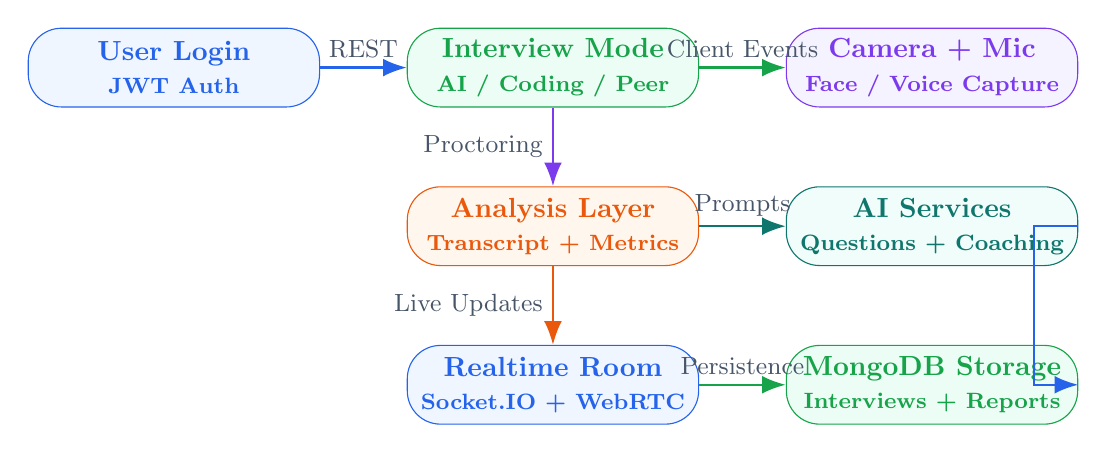
\begin{tikzpicture}[node distance=10mm and 11mm, font=\small]
    \node[draw=PrimaryBlue, fill=SoftBlue, rounded corners=12pt, minimum width=3.7cm, minimum height=1.0cm, align=center, text=PrimaryBlue, font=\bfseries] (login) {User Login\\\footnotesize JWT Auth};
    \node[draw=PrimaryGreen, fill=SoftGreen, rounded corners=12pt, right=of login, minimum width=3.7cm, minimum height=1.0cm, align=center, text=PrimaryGreen, font=\bfseries] (mode) {Interview Mode\\\footnotesize AI / Coding / Peer};
    \node[draw=PrimaryPurple, fill=SoftPurple, rounded corners=12pt, right=of mode, minimum width=3.7cm, minimum height=1.0cm, align=center, text=PrimaryPurple, font=\bfseries] (camera) {Camera + Mic\\\footnotesize Face / Voice Capture};
    \node[draw=PrimaryOrange, fill=SoftOrange, rounded corners=12pt, below=of mode, minimum width=3.7cm, minimum height=1.0cm, align=center, text=PrimaryOrange, font=\bfseries] (analysis) {Analysis Layer\\\footnotesize Transcript + Metrics};
    \node[draw=PrimaryTeal, fill=SoftTeal, rounded corners=12pt, right=of analysis, minimum width=3.7cm, minimum height=1.0cm, align=center, text=PrimaryTeal, font=\bfseries] (ai) {AI Services\\\footnotesize Questions + Coaching};
    \node[draw=PrimaryBlue, fill=SoftBlue, rounded corners=12pt, below=of analysis, minimum width=3.7cm, minimum height=1.0cm, align=center, text=PrimaryBlue, font=\bfseries] (room) {Realtime Room\\\footnotesize Socket.IO + WebRTC};
    \node[draw=PrimaryGreen, fill=SoftGreen, rounded corners=12pt, right=of room, minimum width=3.7cm, minimum height=1.0cm, align=center, text=PrimaryGreen, font=\bfseries] (db) {MongoDB Storage\\\footnotesize Interviews + Reports};

    \draw[-{Latex[length=3mm]}, thick, PrimaryBlue] (login) -- node[above, text=TextMuted] {REST} (mode);
    \draw[-{Latex[length=3mm]}, thick, PrimaryGreen] (mode) -- node[above, text=TextMuted] {Client Events} (camera);
    \draw[-{Latex[length=3mm]}, thick, PrimaryPurple] (mode) -- node[left, text=TextMuted] {Proctoring} (analysis);
    \draw[-{Latex[length=3mm]}, thick, PrimaryTeal] (analysis) -- node[above, text=TextMuted] {Prompts} (ai);
    \draw[-{Latex[length=3mm]}, thick, PrimaryOrange] (analysis) -- node[left, text=TextMuted] {Live Updates} (room);
    \draw[-{Latex[length=3mm]}, thick, PrimaryGreen] (room) -- node[above, text=TextMuted] {Persistence} (db);
    \draw[-{Latex[length=3mm]}, thick, PrimaryBlue] (ai) -- ++(1.3,0) |- (db);
  \end{tikzpicture}%
  }
  \end{figure}

  \vfill
  {\large\textbf{Prepared For:} Project Report, Viva, and Academic Submission\par}
  \vspace{0.2cm}
  {\large\textbf{Note:} This file is separate from project source code and only documents the system.\par}
\end{titlepage}

\tableofcontents
\clearpage

\section{Abstract}
\sectionline
The project presents a full-stack AI-driven interview simulation and recruitment system that combines interview practice, coding assessment, peer collaboration, recruiter evaluation, and personalized career guidance inside a single application. The platform is designed to reduce the gap between theoretical preparation and real interview performance by capturing both technical and communication signals during live interactions.

The system is more than a question-and-answer interface. It creates a structured environment where a user can log in, choose an interview type, speak with an AI interviewer, answer coding tasks, and receive feedback immediately after each response. This makes the platform useful not only for practicing interviews, but also for understanding how performance changes across different question types and time limits.

The application supports multiple real-world scenarios such as mock interviews, coding battles, recruiter assessments, and peer-to-peer practice. It is built to mimic the pressure and flow of an actual interview while still keeping the user inside one simple browser experience.

The backend uses Node.js, Express, MongoDB, and secure JWT authentication, while the frontend uses React, Vite, and Tailwind CSS for a polished and responsive user experience. Browser APIs such as Web Speech API and face analysis utilities are used to capture voice and facial signals in real time. AI services generate the interview flow and feedback, making the system useful for candidates, educators, and recruiters.

The overall outcome is a practical learning and recruitment platform that helps users improve both technical accuracy and communication quality. It also gives recruiters and teachers a repeatable way to evaluate candidates using the same workflow every time.

\clearpage

\section{Problem Statement}
\sectionline
Traditional interview preparation is fragmented. Students practice coding on one site, spoken answers on another, and live interview behavior in a completely different environment. Recruiters often depend on manual observation, scattered notes, and disconnected tools for video, code, and assessment. This makes the process expensive, slow, and inconsistent. A candidate may solve the technical problem but still fail because of communication issues, lack of eye contact, or poor confidence, yet such issues are rarely measured objectively.

There is also a growing need for systems that can scale across multiple interview formats. Technical interviews require coding sandboxes and test-case evaluation. Behavioral interviews require dynamic question flow and answer tracking. Peer and competitive modules require realtime synchronization. Career planning needs personalized recommendations. The absence of one integrated platform creates friction for both learners and hiring teams.

From a user perspective, the biggest gap is feedback quality. Most tools only show whether an answer was correct or incorrect, but they do not explain how the candidate spoke, how confidently they responded, or how they handled pressure. This means learners often repeat the same mistakes without knowing what to improve.

From an organizational perspective, interview data is often stored in separate places and is difficult to compare across candidates. That limits consistency and makes it hard to build a reusable evaluation process. A more complete platform should combine authentication, realtime interaction, scoring, reports, and learning guidance in one place.

This project addresses these problems by bringing all the required workflows into one application. It uses AI to generate interview content, browser intelligence to measure delivery signals, and structured storage to preserve session history and reports.

\clearpage

\section{Difference Between Traditional and Modern Approach}
\sectionline
\begin{table}[H]
\centering
\renewcommand{\arraystretch}{1.25}
\begin{tabularx}{\textwidth}{>{\raggedright\arraybackslash}p{3.2cm} >{\raggedright\arraybackslash}X >{\raggedright\arraybackslash}X}
\toprule
\rowcolor{SoftBlue}
\textbf{Aspect} & \textbf{Traditional Interview Flow} & \textbf{This Project} \\
\midrule
Preparation & Separate coding practice and mock interview tools & One unified system with AI coaching, coding, and mock interviews \\
Evaluation & Manual notes and subjective judgment & AI-based response scoring with voice and facial analytics \\
Question flow & Static or prewritten questions & Adaptive next-question generation based on performance \\
Live coding & External editor or shared document & Embedded Monaco editor with run and submit workflow \\
Feedback & Delayed and generic & Immediate report with structured metrics and summaries \\
Collaboration & Email or video meeting only & Peer mock interviews and realtime battle rooms \\
\bottomrule
\end{tabularx}
\end{table}

The modern approach improves consistency and usability. Candidates get a realistic practice environment, while recruiters and instructors receive measurable evidence instead of only impressions. The same platform can support practice, hiring, and learning guidance without requiring the user to switch between multiple unrelated services.

\clearpage

\section{Proposed Solution}
\sectionline
The proposed solution is a modular, browser-centric interview platform that behaves like a professional online assessment environment. It is divided into a frontend experience layer, a backend orchestration layer, a database persistence layer, and an AI decision layer. The frontend presents the interview workspace, recruiter portal, coach, roadmaps, and coding interface. The backend secures all flows, coordinates AI calls, and stores interview records. The database keeps user profiles, interview sessions, code submissions, reports, and roadmap data. AI services generate adaptive content and feedback.

The platform supports multiple user journeys. A candidate can sign in, choose an interview type, start a live session, answer the AI interviewer, submit code, and review the feedback report. A peer can enter a mock room and practice with another user. A recruiter can schedule sessions and review performance. A learner can open the coach and receive a roadmap that suggests what to study next. Because all of these experiences use the same authentication and storage foundation, the system stays consistent and maintainable.

A key strength of the solution is that it combines technical evaluation with communication analysis. Instead of measuring only correctness, it also considers pace, confidence, face detection, and fluency. This produces a richer interview report and helps users improve in a practical way.

\clearpage

\section{Overall Architecture}
\sectionline
\subsection{High-Level Architecture Diagram}
\begin{figure}[H]
\centering
\resizebox{0.96\textwidth}{!}{%
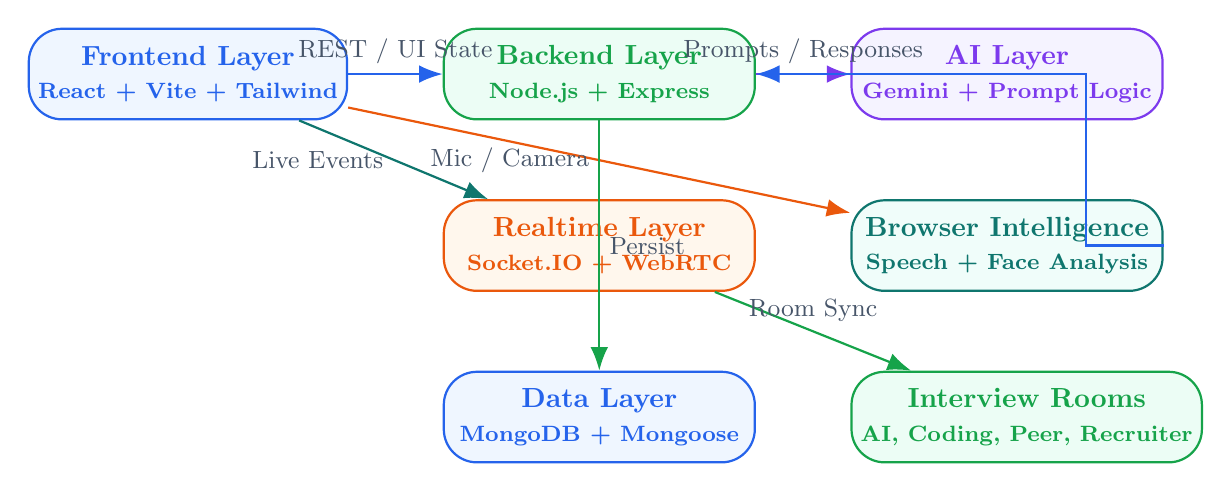
\begin{tikzpicture}[node distance=10mm and 12mm, font=\small]
  \node[draw=PrimaryBlue, fill=SoftBlue, rounded corners=12pt, thick, minimum width=3.95cm, minimum height=1.15cm, align=center, text=PrimaryBlue, font=\bfseries] (frontend) {Frontend Layer\\\footnotesize React + Vite + Tailwind};
  \node[draw=PrimaryGreen, fill=SoftGreen, rounded corners=12pt, thick, right=of frontend, minimum width=3.95cm, minimum height=1.15cm, align=center, text=PrimaryGreen, font=\bfseries] (backend) {Backend Layer\\\footnotesize Node.js + Express};
  \node[draw=PrimaryPurple, fill=SoftPurple, rounded corners=12pt, thick, right=of backend, minimum width=3.95cm, minimum height=1.15cm, align=center, text=PrimaryPurple, font=\bfseries] (ai) {AI Layer\\\footnotesize Gemini + Prompt Logic};
  \node[draw=PrimaryOrange, fill=SoftOrange, rounded corners=12pt, thick, below=of backend, minimum width=3.95cm, minimum height=1.15cm, align=center, text=PrimaryOrange, font=\bfseries] (realtime) {Realtime Layer\\\footnotesize Socket.IO + WebRTC};
  \node[draw=PrimaryTeal, fill=SoftTeal, rounded corners=12pt, thick, right=of realtime, minimum width=3.95cm, minimum height=1.15cm, align=center, text=PrimaryTeal, font=\bfseries] (browser) {Browser Intelligence\\\footnotesize Speech + Face Analysis};
  \node[draw=PrimaryBlue, fill=SoftBlue, rounded corners=12pt, thick, below=of realtime, minimum width=3.95cm, minimum height=1.15cm, align=center, text=PrimaryBlue, font=\bfseries] (db) {Data Layer\\\footnotesize MongoDB + Mongoose};
  \node[draw=PrimaryGreen, fill=SoftGreen, rounded corners=12pt, thick, right=of db, minimum width=3.95cm, minimum height=1.15cm, align=center, text=PrimaryGreen, font=\bfseries] (rooms) {Interview Rooms\\\footnotesize AI, Coding, Peer, Recruiter};

  \draw[-{Latex[length=3mm]}, thick, PrimaryBlue] (frontend) -- node[above, text=TextMuted] {REST / UI State} (backend);
  \draw[-{Latex[length=3mm]}, thick, PrimaryPurple] (backend) -- node[above, text=TextMuted] {Prompts / Responses} (ai);
  \draw[-{Latex[length=3mm]}, thick, PrimaryOrange] (frontend) -- node[left, text=TextMuted] {Mic / Camera} (browser);
  \draw[-{Latex[length=3mm]}, thick, PrimaryGreen] (backend) -- node[right, text=TextMuted] {Persist} (db);
  \draw[-{Latex[length=3mm]}, thick, PrimaryTeal] (frontend) -- node[left, text=TextMuted] {Live Events} (realtime);
  \draw[-{Latex[length=3mm]}, thick, PrimaryGreen] (realtime) -- node[above, text=TextMuted] {Room Sync} (rooms);
  \draw[-{Latex[length=3mm]}, thick, PrimaryBlue] (browser) -- ++(1.0,0) |- (backend);
\end{tikzpicture}%
}
\caption{High-level architecture of the system}
\end{figure}

\subsection{Architecture Explanation}
\begin{enumerate}
  \item \textbf{Frontend:} React components render the interview setup, live session, dashboard, battle, coach, recruiter, and peer pages. The UI is kept responsive with Tailwind utility classes.
  \item \textbf{Backend:} Express controllers manage authentication, session creation, question generation, code execution requests, and report generation.
  \item \textbf{AI Services:} The system uses a prompt-based service layer to generate interview questions, adjust difficulty, and summarize coaching feedback.
  \item \textbf{Browser Intelligence:} The client captures mic and camera data locally, enabling transcript generation and facial analysis without uploading raw video frames.
  \item \textbf{Database:} MongoDB stores the evolving interview state, user reports, roadmap progress, peer invitations, and recruiter workflows.
\end{enumerate}

The architecture is intentionally split into clear layers so that the interface can remain fast while the backend handles security and orchestration. This separation also makes the project easier to extend with new interview types or learning modules in the future.

\clearpage

\section{Technologies Used}
\sectionline
\begin{table}[H]
\centering
\renewcommand{\arraystretch}{1.25}
\begin{tabularx}{\textwidth}{>{\raggedright\arraybackslash}p{3.2cm} >{\raggedright\arraybackslash}X}
\toprule
\rowcolor{SoftGreen}
\textbf{Technology} & \textbf{Purpose in the Project} \\
\midrule
React + Vite & Fast frontend rendering, routing, and component-based UI \\
Tailwind CSS & Modern styling for dashboards, forms, cards, and responsive layouts \\
Node.js + Express & REST API layer, interview orchestration, and secure server logic \\
MongoDB + Mongoose & Persistent document storage for users, questions, answers, and reports \\
Google Gemini API & Dynamic question generation and AI-driven feedback \\
Socket.IO & Realtime updates for battle rooms and peer sessions \\
WebRTC & Peer-to-peer audio and video communication \\
Web Speech API & Speech recognition for interview answer capture \\
face-api.js & Browser-side facial analysis and proctoring signals \\
Monaco Editor & Professional coding workspace for coding interviews \\
\bottomrule
\end{tabularx}
\end{table}

\subsection{Technology Justification}
React and Vite are used because the project has many interactive screens and state transitions. Tailwind CSS gives a clean interface without large custom style sheets. Node.js and Express make it easy to build secure APIs and connect to AI services. MongoDB fits the nested interview and response data model. Socket.IO and WebRTC are ideal for live interactions and synchronized interview rooms. The browser speech and face APIs reduce the need for external services and keep the user experience real-time.

These technologies together allow the system to support live interviews, peer rooms, coaching, coding battles, and recruiter workflows without changing the project architecture for each new feature.

\clearpage

\section{Module-Wise Description}
\sectionline
\subsection{Authentication Module}
The authentication module manages registration, login, email verification, forgot password, and reset password workflows. It uses secure credential handling and protects the rest of the platform through authenticated routes. This module is important because every other feature depends on user identity and access control.

\subsection{AI Interview Module}
This module powers the interview setup page, the live question flow, the adaptive follow-up behavior, and the final report generation. It sends prompts to the AI service and stores answers and evaluations in the database. The module also uses timing logic so that questions are displayed one at a time and the interview can progress naturally.

\subsection{Coding Interview Module}
The coding module combines a problem statement panel, a language selector, a Monaco editor, run and submit buttons, and test-case results. Users can solve algorithmic problems in a coding environment that looks and behaves like a lightweight online judge.

\subsection{Coach and Roadmap Module}
The coach module provides chat-based guidance, while the roadmap module produces personalized learning pathways. Both modules help users understand what to improve and which topics to focus on next.

\subsection{Peer and Battle Module}
The peer module is intended for user-to-user practice, while the battle module simulates competitive coding. These features help learners practice under pressure and collaborate with others.

\clearpage

\section{Agents Used}
\sectionline
\begin{itemize}
  \item \textbf{AI Interviewer Agent:} Generates interview questions and adapts the next question based on the candidate response.
  \item \textbf{AI Evaluator Agent:} Scores the response using transcript quality, communication style, and task completion.
  \item \textbf{AI Coach Agent:} Replies to career questions and suggests what the user should learn next.
  \item \textbf{Proctoring Agent:} Monitors face presence, eye direction, and other browser-level integrity signals.
\end{itemize}

The agents work together to simulate a realistic interview session. Instead of giving static responses, they react to the user's context, progress, and performance.

\subsection{Agent Interaction Flow}
\begin{enumerate}
  \item The user opens an interview or coach session.
  \item The backend sends context to the AI service.
  \item The AI returns structured JSON or generated text.
  \item The frontend displays the response and updates the session state.
  \item The evaluator and proctoring logic store analytics and feedback.
\end{enumerate}

\clearpage

\section{Algorithms Used}
\sectionline
\begin{itemize}
  \item \textbf{Adaptive Question Sequencing:} The system chooses the next question based on the candidate's previous answer quality and interview history.
  \item \textbf{Similarity Filtering:} Generated questions are compared against previous prompts to avoid repetition or near-duplicate content.
  \item \textbf{Speech Transcript Aggregation:} Interim and final speech chunks are merged so that long answers are captured reliably.
  \item \textbf{Biometric Smoothing:} Expression and eye-contact data are smoothed across frames before a final score is shown.
  \item \textbf{Code Evaluation Flow:} Candidate code is executed against defined test cases and the result is stored for later review.
\end{itemize}

\subsection{Why These Algorithms Matter}
The AI interview flow depends on variation and continuity. Repetition makes the experience feel unnatural, while over-aggressive submission can cut off a candidate's response. The project therefore combines timing logic, transcript buffering, question similarity checks, and evaluation routines to make the experience feel more human and more reliable.

\subsection{Simple Pseudocode Summary}
\begin{verbatim}
if answer is short and speech stops:
    wait a few seconds
    submit response automatically
if AI question is too similar:
    replace it with a safer fallback question
if candidate is coding:
    show test cases and wait for manual submit
\end{verbatim}

\clearpage

\section{Database Design and API Summary}
\sectionline
The backend stores users, interviews, responses, roadmaps, resumes, recruiter sessions, peer invitations, and battle state in MongoDB. This structure allows the application to keep historical records and generate reports later.

\begin{table}[H]
\centering
\renewcommand{\arraystretch}{1.25}
\begin{tabularx}{\textwidth}{>{\raggedright\arraybackslash}p{3.8cm} >{\raggedright\arraybackslash}X}
\toprule
\rowcolor{SoftBlue}
\textbf{Collection / Model} & \textbf{Stored Information} \\
\midrule
User & Authentication data, profile details, role, email verification state \\
Interview & Setup, questions, responses, scores, report state \\
Resume & Parsed resume text and uploaded file metadata \\
Roadmap & Personalized learning nodes, topics, progress state \\
PeerInterview & Peer room metadata, participants, status, feedback \\
Battle & Competitive coding room data, players, score state, result \\
RecruiterInterview & Recruiter session setup, code, rubric, evaluation \\
\bottomrule
\end{tabularx}
\end{table}

\subsection{Representative API Groups}
\begin{itemize}
  \item Authentication: login, register, verify email, forgot password, reset password
  \item Interview: create session, get session, submit answer, skip question, complete interview
  \item Code: run code against test cases and return execution results
  \item Coach: ask questions, receive roadmap suggestions, store chat history
  \item Recruiter and Peer: manage rooms, invitations, schedules, and candidate sessions
\end{itemize}

The API structure is split by feature so that the frontend can request only what it needs. This keeps the interface responsive and the backend maintainable.

\clearpage

\section{Security and Scalability}
\sectionline
Security is critical because the platform handles user accounts, interview sessions, video streams, and AI prompts. Passwords are hashed, JWTs protect private routes, and the browser keeps raw webcam data local. The server validates inputs so that malicious or malformed requests do not break the workflow.

Scalability matters because the platform supports realtime rooms and AI-generated responses. Socket.IO and WebRTC reduce server load for live media traffic. MongoDB stores documents flexibly, which is useful for nested interview analytics. The AI layer is isolated on the backend, so credentials are not exposed to the browser.

\subsection{Security Measures}
\begin{itemize}
  \item JWT authentication for protected pages and API routes
  \item Password hashing before storage
  \item Backend-only AI API calls
  \item Client-side face analysis instead of raw video upload
  \item Validation and centralized error handling
\end{itemize}

\subsection{Scalability Measures}
\begin{itemize}
  \item Independent frontend and backend deployment
  \item Realtime communication using lightweight events
  \item Flexible MongoDB schema for future feature growth
  \item Modular feature folders for easier maintenance
\end{itemize}

\section{Implementation Phases and Testing}
\sectionline
\subsection{Implementation Phases}
\begin{enumerate}
  \item \textbf{Foundation:} Authentication, routing, environment variables, and database connection.
  \item \textbf{Interview Core:} Interview setup, live question flow, answer capture, and report generation.
  \item \textbf{Coding Workspace:} Problem statements, Monaco editor, run and submit flow, test-case display.
  \item \textbf{Realtime Features:} Battle rooms, peer mock interview rooms, and schedule management.
  \item \textbf{AI Coach and Roadmaps:} Career guidance, roadmap generation, and chat interface.
  \item \textbf{Final Polish:} Dashboard, analytics, response handling, and UI consistency.
\end{enumerate}

\subsection{Testing Approach}
\begin{itemize}
  \item Authentication flow testing for login, register, and email verification
  \item Interview flow testing for question generation and answer submission
  \item Speech recognition testing for long and short responses
  \item Code execution testing using sample problems and hidden cases
  \item UI testing for responsiveness on laptop and mobile viewports
\end{itemize}

\subsection{Typical Validation Scenarios}
\begin{longtable}{p{5cm}p{9cm}}
\toprule
\rowcolor{SoftGreen}
\textbf{Scenario} & \textbf{Expected Result} \\
\midrule
User logs in successfully & Dashboard opens and protected routes become accessible \\
Interview question is displayed & Avatar speaks once and the chat shows the current prompt \\
Candidate speaks long answer & Transcript keeps collecting final chunks without cutting off early \\
Coding solution is submitted & Backend evaluates code and returns results with test-case outcome \\
Question is repeated by model & Fallback question replaces the duplicate prompt \\
\bottomrule
\end{longtable}

\clearpage

\section{Applications and Future Scope}
\sectionline
\subsection{Applications}
\begin{itemize}
  \item \textbf{Students and Job Seekers:} Practice interviews, improve communication, and solve coding questions.
  \item \textbf{Teachers and Bootcamps:} Assign mock interview exercises and review analytics.
  \item \textbf{Recruiters:} Schedule and run structured interviews with scoring support.
  \item \textbf{Peer Practice Groups:} Use peer rooms to simulate human-led interviews.
  \item \textbf{Competitive Coders:} Use battle mode for speed, accuracy, and pressure practice.
\end{itemize}

\subsection{Future Scope}
The platform can be extended in several directions. A multi-language voice output system can improve accessibility. A richer analytics dashboard can show trends over time. The code engine can be integrated with more execution languages or container-based sandboxes. The peer network can support larger rooms and advanced matchmaking. The roadmap system can become more personalized by using resume insights, past performance, and user preferences.

\subsection{Why This Project Matters}
The system helps users prepare in a realistic environment rather than only reading theory. It also gives recruiters and educators a repeatable way to assess candidate skills. That combination makes the platform useful across both learning and hiring contexts.

\clearpage

\section{Conclusion}
\sectionline
The AI-Driven Interview Simulation and Recruitment System is a practical and modern platform for technical assessment, guided practice, and career preparation. It brings together live interview flow, coding assessment, peer sessions, competitive practice, and AI coaching in a single application. The system reduces fragmentation, improves feedback quality, and provides measurable signals about both technical and communication performance.

By combining React, Node.js, MongoDB, WebRTC, Socket.IO, speech recognition, facial analysis, and AI-driven generation, the project demonstrates how a real-world interview environment can be modeled inside the browser. The resulting platform is scalable, maintainable, and relevant to students, developers, educators, and recruiters.

\clearpage

\section{References}
\sectionline
\begin{enumerate}
  \item React Documentation: \url{https://react.dev/}
  \item Node.js Documentation: \url{https://nodejs.org/api/}
  \item Express Documentation: \url{https://expressjs.com/}
  \item MongoDB Documentation: \url{https://www.mongodb.com/docs/}
  \item Mongoose Documentation: \url{https://mongoosejs.com/docs/guide.html}
  \item Socket.IO Documentation: \url{https://socket.io/docs/v4/}
  \item WebRTC API Reference: \url{https://developer.mozilla.org/en-US/docs/Web/API/WebRTC_API}
  \item Web Speech API Reference: \url{https://wicg.github.io/speech-api/}
  \item face-api.js Documentation: \url{https://justadudewhohacks.github.io/face-api.js/docs/index.html}
  \item Monaco Editor: \url{https://microsoft.github.io/monaco-editor/}
  \item Google Gemini API: \url{https://ai.google.dev/}
\end{enumerate}

\vfill
\begin{center}
  {\small\color{TextMuted}Standalone documentation file created for the project. Project source code remains unchanged.}
\end{center}

\end{document}




